\chapter{Background}

It would right if we start the book with the article \cite{intro} that was the first on the way to Novoslovnica construction.

The Slavic world has a deep and rich history. The Slavic tribes appeared on the vastness of Europe, and during their history of growth and development they have reached an extraordinary territorial vastness of settlement. We can say that the formed tribes of the Slavs lived on a huge territory according to Europe standards: from the Elbe in the West to the Volga in the East, from the Aegean sea in the South to the Neva river in the North. Further, due to the development of Kievan Rus and the Russian state, the Slavs settled throughout Eastern Europe and Siberia. Despite all the contradictions in politics and strife, the cultural and linguistic component of the Slavs continued to be preserved. Of course, the tribes bordering on other Nations have experienced enormous cultural and linguistic pressure, including Turkic, Roman, Finno-Ugric peoples.

Despite this, the Slavs retained their cultural identity and mentality. So, we can easily understand a person from the same group (Eastern, Western, Southern) and with little difficulty can establish communication with a person from another group of Slavs. This gives us the right to talk about the brotherhood of the Slavic peoples.

Many of the Slavic peoples have sunk into Oblivion, some in very recent times. For example, the POLAB culture left with the language by the middle of the 20th century. However, most of them remained alive, and from our common efforts depends on what will be the future of the Slavs.

From modern Slavic peoples only East Slavic group had relative stability and self-sufficiency. Russian experienced several waves of foreign language intervention — Mongolian, German, French and English, from which he, generally speaking, came out the winner, in many cases enriching and diversifying its vocabulary. At the moment, the English intervention, the strongest since the Tatar-Mongolian yoke, which has withdrawn many native Russian words from our everyday life, has not ended. But Slavs do it, assimilating came, and sometimes returning lost.

The situation is different in other Slavic groups. Not possessing constant sovereign statehood, Western and Eastern Slavs were subject to constant influence other peoples. Thus, the intervention of the Turkish language in the South Slavic languages and culture can be correlated with the Tatar-Mongolian yoke for Russia. After liberation from Turks, southern Slavs have become to experience Western influence, and we can to see enough a large number of borrowing from English, French and camping on p. in Bulgarian and Serbian languages.

Throughout its history, Western Slavs were constantly terrorized by the influence of Romanesque languages. So, under the onslaught of the Germans, the Slavs lost their land along the Elbe and retreated to the Oder. Thus, the influence of the Romanesque tribes was also facilitated by the adoption of the Latin alphabet by the languages of the Western Slavs, instead of a possible Glagolitic or Cyrillic. Anyway, Slavs, though, and have undergone numerous impacts on their culture, managed to keep a common language to the present day.

The problem of reconsolidation of the Slavic peoples worried all many centuries ago and attempts were made to implement it. This can be considered the creation of Kievan Rus, the Grand Duchy of Lithuania, the expansion of the Russian Empire to the West, the creation of friendly relations with the Balkans, the creation of ATS, Yugoslavia, Czechoslovakia. However, the problem of the impossibility or short-lived nature of this Union arose not because of the establishment of friendly, fraternal relations, but the prevalence of the interests of one nation over all the other members of the Union, which inevitably led to the collapse and failure.

There is a fair idea that the inability to undertake such an Association is not only in the political interests of any country, Yes, undoubtedly, but also in the language of communication, state or Union language. It is impossible to make official all languages and adverbs existing in any district, and declaring one language more important than another we want this or not we turn ourselves to the further collapse of such relations.

The necessity and importance of the creation of the Slavic (pan-Slavic) language was realized in the 16th century, when the first attempts were made to create a common language for all Slavs. However, they did not bring the expected results and sank into oblivion.

Most recent developments of pan-Slavic languages are based on the principle of simplification, minimizing all vocabulary and grammar of languages. For example, these Words and Mezhduslovnyh English Wuhan. We believe this is fundamentally wrong, as the new language should not be aimed at the degradation of cultures, but rather to maintain the grandeur and beauty of Slavic culture and identity. Therefore, our principle is not to "Discard all that is foreign", but to "Unite all the best".

If we analyze why the Slavs need a new Slavic language, we can distinguish several positions:

\begin{itemize}
	\item the need for an additional consolidating factor to unite the policy of the Slavic peoples.
	\item The need to strengthen mutual understanding and improve the Slavs ' perception of each other.
	\item Preserve the original richness and beauty of all Slavic languages.
	\item The impossibility of taking the role of the Slavic language of Russian (and Polish) due to historical reasons.
	\item Inability to accept the role of the Slavic language of the previous planned projects in full due to objective reasons.
\end{itemize}

\section{Historical background}

Baltic scientists in their research \cite{slavic-procent} worked out a model of Slavic lexical identity. In the picture, you can see the percentage of common lexicon provided by connections between different Slavic languages.

There are three Slavic linguistic and ethnic branches - East Slavic (Russian, Belorussian, Ukrainian and Rusyn), West Slavic (Czech, Slovak, Polish, Kashubian, Silesian, Upper-Sorbian, Lower-Sorbian) and South Slavic (Slovenian, Serbian, Croatian, Macedonian and Bulgarian).

This division goes back into history. Different communication events with other nations, geographical position, territorial pecularity - everything affected Slavic people that became nations that now exist. It is supposed to have three initial tribes of Slavs: Venedes (the ancestors of West Slavs), Antes (the ancestors of East Slavs) and Sklavins (the ancestors of South Slavs). It is controversial, but a viable and a rather popular model within Slavic community.

\begin{figure}
	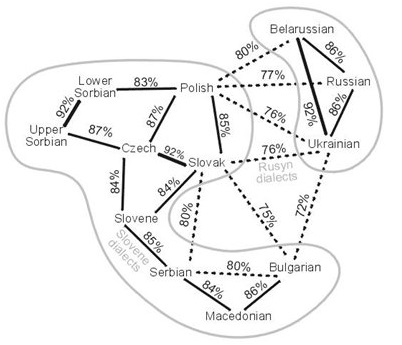
\includegraphics[width=\linewidth]{./sources/percents.jpg}
	\caption{Lexicon connections in Slavic languages}
	\label{fig:percent}
\end{figure}

Nevertheless, Slavs started to separate from each other in the seventh century. South Slavs came to Balkan peninsula and assimulated the Illyrian and Turkic peoples that lived there already. Thus, we see how Croatians and Bulgars appeared. The confrontation of Slavs and Germans lead to West Slavic peoples' appearance. Spreading to the East and confrontation with Finno-Ugric and Turkic peoples poured out into the appearance of East Slavic nations.
\section{Script background}

One of the Central ideas of pan-Slavism is the creation of a common Slavic language. This problem was solved many times in one form or another and in different ways starting with the old Church Slavonic language created by St. brothers Constantine-Cyril and Methodius. The invention of the first common Slavic language is associated with the appearance of the first writing, which was to become common Slavic — Glagolitic.

However, over time, the part of the Slavs adopted the Cyrillic alphabet, the piece took Latin, and some for a while had the Glagolitic alphabet, the Latin alphabet and a modified Cyrillic alphabet, known as bosancica or horvatica (there are other names). Glagolitic also changed, becoming from rounded "Bulgarian" an angular "Croatian". But the main thing was — the language itself changed. Once a common old Church Slavonic began to divide into version that started to converge with the live Slavic languages. We can name some version of Church Slavonic: Russian Slavonic, Bulgarian Slavonic, Serbian Slavonic, Croatian Slavonic etc.

Attempts to solve the problem of separation of Slavic languages and scripts gave several options:

\begin{itemize}
	\item To revive the Church Slavonic language anyhow with adding elements of live languages to it or without adding.
	\item Take one of the live languages, but with certain modifications — adding new letters or words from other Slavic languages, new grammatical structures and so on.
	\item As in the previous item, but do not change anything and try to spread the live language through educational courses and other forms of education.
	\item As in the previous point, but forcibly.
	\item Create a new artificial / semi-artificial language based on those elements of the Slavic languages that remain common or can be relatively easily reduced to common + a number of different elements, to facilitate the "entry" into the language of the Slavs who speak different Slavic languages, or on the basis of only common elements.
\end{itemize}

The second part of the problem is writing. Due to the fact that the Glagolitic alphabet and bosancica virtually disappeared and remained only in limited use (bosancica disappeared almost completely, and the Glagolitic alphabet is supported in Croatia), the remaining candidates for the Slavic alphabet stays Cyrillic and Latin.

Generally, it can be said that new interslavic projects often use the Latin alphabet that cuts obsessiveness of these projects, because Cyrillic and Latin alphabets still are native to Slavic writing systems:

\begin{itemize}
	\item in one case, a literature began almost immediately with the Latin alphabet
	\item in the other a literature started with the Cyrillic alphabet
	\item somewhere both Latin and Cyrillic scripts are used
	\item somewhere the transition from Cyrillic to Latin script took place
\end{itemize}

In Yugoslavia, Cyrillic and Latin tried to lead to a common denominator through the creation of the so-called Slavica. The essence of Slavica was to leave the backbone of the Latin alphabet (all the basic letters + letters, the same for the Latin and Cyrillic), replace all the digraphs, letters with diacritics and digraphs with diacritics corresponding Cyrillic letters. In Yugoslavia, this was all the easier to do because the Yugoslav Cyrillic and Latin alphabet are completely identical in composition having a mutual transliteration of each other. However, this project failed because of the resistance of nationalists in Croatia.
\section{Interslavic background}

We all know that the idea of a common language for the Slavs hovers among the Slavic peoples for more than a Millennium. The first and only successful project to date was the Church Slavonic language of Cyril and Methodius. This language has successfully found its niche in religious use and is used with some changes to the present day. However, such attempts for the secular language were resumed only in the 17th century in the works \cite{krizhanich} \cite{matija}. Moreover, the working project was neither created nor introduced into society, while some similar projects of planned languages for romance languages have successfully taken root and found a wide response in society (Esperanto, Interlingua).

The revival of the idea of the inter-Slavic language in our days occurred in 1999, when mark Gucco from Slovakia created the language of Slovio. This language has a huge number of shortcomings and is currently not recognized as capable by any of the developers of the inter-Slavic project, but it served as a catalyst for the emergence of a large number of such projects and the development of the idea of creating a planned inter-Slavic language that could meet the needs of modern society. 

After that, more than 20 similar projects, more or less developed, appeared in 10 years. In 2006 there was a project slavianski, created (Ondrej Rečnik and Gabriel Svoboda). This language was developed in parallel in different degrees of detail, he put his ideas Jan van Steenbergen and Igor Polyakov. In 2009, the project broke away from the project Slovioski (Steeven Radzikowski, Andrej Moraczewski and Michal Borovička), which tried to unite the ideas of Slovio and Slovyanski. However, in 2010, all these projects were merged into one under the name Interslavic (see below - Interslavic-2).

At the same time, the Czech programmer Vojtěch Merunka published under the name of Neoslavonic. This project suggested the idea of how the Church Slavonic language could develop in free development. In 2011, these two projects began cooperative work on a common case. (see figure 1) then, this project has taken a leadership position on the issue of building medullablastoma language. Only in 2012 there was one project of “Northern Slavic language” (Venedčyna), presented by Nikolai Kuznetsov, who then joined Interslavic, and in 2014 there was a project of Novoslovnitsa, presented by George Carpow and the development team mainly from the countries of Eastern and southern Slavs, which at the moment remains the only living independent project outside the project Interslavic.

Interslavic introduced the idea of flavorisation, which resulted in a valid language differentiation of dialects and spellings and the lack of codification. In 2017, the project Neoslavonic and Interslavic merged into a new project called interslavic-2, which was a compromise between the ideas of Vojtěch Merunka and Jan van Steenbergen (who headed the project interslavic-1). They presented their new ideas in the article \cite{interslavic-2}, which was published in July 2017.

